% THESIS CHAPTER

\chapter{Software architecture}
\label{chap:sixth
}
\ifpdf
    \graphicspath{{Chapter6/Figures/PNG/}{Chapter6/Figures/PDF/}{Chapter6/Figures/}}
\else
    \graphicspath{{Chapter6/Figures/EPS/}{Chapter6/Figures/}}
\fi

% short summary of the chapter
\section*{Summary}

This Chapter introduces the reader to the software architecture running off board on Linux. The introduction presents a  general overview on software architectures, expressed the needs of such a system and in particular it describes the environment and software tools involved. Next section presents the design pattern according to which the software is organized explaining its advantages and limitations. Then the software components are described with more detail one by one and the results of the experiments are reported. 
\section{Introduction to the proposed architecture}

Architecture is usually intended as the process or product of planning, designing and constructing entities. Usually those entities refer to buildings and structure but the concept can be extended to vehicles, electrical and electronics components or softwares. The architect decides where to locate different elements such as walls, doors columns and windows and connect them in harmony with structural consistency. In the same way the software engineer connect, design and locate different software components. A component could be a program implementing an algorithm, some conversion or a graphical user interface. The basic idea of architecture definition is to design software structure and object interaction before the detailed design phase. Although serious architecture definition is being suggested for large projects only, arguably any software construction or implementation work must be preceded by an architectural design \cite{msdn}.
 \subsection{Motivations}
At this point one may ask: why do we need to define an architecture? The answer is pretty simple: it makes things easier,more clear and simpler. A software architecture is an abstract view of a software system distinct from the details of implementation, algorithms, and data representation. Thus it gives an organizational map we may follow during the design flow. A well written software architecture should:
 \begin{itemize}
 \item Provide flexibility and adaptability.
 \item Allow for interoperability with other softwares and elements in general.
 \item Provide control on the system.
 \item Reduce maintenance time and cost.
 \item Help developers improving the software.
 \end{itemize}
Reusability is a key aspect in design of this kind of systems. One software may be used for a different application changing only few parameters or modules. Each module should be self contained and work as a \textit{black box}, meaning that once the input and output are defined, the actual implementation has no importance. Standardization clearly takes an important role, the way components communicate for example must be known by the developer. If different modules speak the same \textit{language} or \textbf{protocol} (e.g. the MavLink standard) in engineering terms, it is simpler to interface them. Moreover, a self contained module is more easy to maintain and expand because developers can focus on that specific aspect without knowing what is happening outside. In that way specialist in different fields can cooperate designing each own part. The role of the software engineer is on one hand to design software components, and on the other to integrate them with modules written by others. Finally, it seems trivial to point it out, but the architecture must work respecting the specifications and providing the needed control on the system. 

\paragraph{Note:}This software was designed ad-hoc for indoor flight because there were not any other alternatives. Every control station is specialized for outdoor flight which is not our case. Moreover this software aims to become a research platform for controlled environments (e.g. indoor flight) for anyone who wants to contribute.
\subsection{Programming environment and tools}

Every job has its own tools. In order to implement what we theorized in the introduction of this Chapter we need to rely on software tools. There are many different frameworks which helps developers in implementing their own ideas.

 The state of the art and widely used framework in robotics is ROS or Robotic Operative System \cite{ROS}. ROS is a publish/subscrbe middleware meaning that it packs function classes and features which provide inter process communication. It supports most of the libraries used in robotics for path planning, computer vision, control and so on. The main feature is that ROS is very easy to use and let the user create different parallel processes (or nodes) without focusing on low level aspects. As consequence of that, the designer can concentrate on the actual problem he is working on and leave lower level managing such as shared variables, timing or buffers to ROS. This feature increase exponentially the productivity while writing a program. Moreover, ROS is becoming a standard in research and also industry. That means that many packages are available online that one can use, the community and the documentation are superb and it is open source. This framework has all the features needed for a good base of a software architecture.
 
 However there are three main reason which made me discard ROS as a choice. First of all, as stated in Chapter \ref{chap:second}, most of the control stations are written with Qt libraries. Since one may thing to include this architecture in one of them in the future, could be an idea to go in the same direction. The second one is that the very first module of this architecture was written by a PhD student, Tommaso Falchi Delitalia, using the Qt framework. It was nice to have a base starting point and expand from that. The last reason, but not the least, is that ROS gave me important delay problems when I tried to integrate mavlink in it. Mavlink is not fully supported but some packages, in development, are out there and they simplify the design such as the acquisition of data from Motive \cite{optiros}.

Hence the used tools are \textbf{Qt libraries} \cite{qt} while the chosen programming language is C++, widely used and a standard in robotics. Qt is a powerful framework that let the user create user interfaces with good performance. It packs a set of classes, functions and libraries for almost any kind of needs. Moreover is portable on different platforms such as tablets, smartphones and the most important operative systems. for this reason it is used to implement control station, applications like navigators and vehicles control panels.

The functions and classes used for this project are debugging functions to print logs, multi-threading classes to implement parallel modules, sockets interfaces classes and system functions to manage lower level services.By far Qt seems perfect, it provides a very easy access to many features, the documentation is very clear and the learning time is pretty low. The very big disadvantage is the lacking of inter process communication support. The pub/sub design is perfect for robotics application but Qt does not provide any help on that, at least for now. Thus the drawbacks of using this kind of framework is that we need to manage inter process message pass-through in some way. This is done and explained in section \ref{sec:sofdescrip}. A porting on ROS could be interesting in the future, after solving delay related issues, for research interests.
\section{Design patterns}
\label{sec:patterns}
In the course of history the concept of \textit{style} was born and developed. An architectural style is characterized by the features that make a building or other structure notable and historically identifiable. The style identifies a common trend, elements or rules that are used in a particular period or by a group of people during the design flow. The same concept evolved to various disciplines; in computer science, the architecture "style" is often called \textbf{Design Pattern}. The analogy with building design is strong, the formal definition of design pattern is the following: 
\paragraph{Definition of Design Pattern}:  \textit{a design pattern is a general reusable solution to a commonly occurring problem within a given context in software design.} \\

\noindent
The pattern is a description or template for how to solve a problem that can be used in many different situations, usually for groups of problems. Similarly to the architecural style, the software pattern is defined by common structures, participants, communications, protocols and standards. Design patterns can speed up the development process by providing tested, proven paradigms. Thus the software architecture is defined by its style, namely design pattern, which is chosen among the available ones. First step to follow during the prototyping of the software is to have clear in mind which kind of problem we are facing and which are the constraints of the system. 

At this point the reader should ask how is the software interfacing with the robot and which kind of control does it have on the system. As stated in Chapter \ref{chap:fifth}, the external signals that are input of the on board flight stack are the 4-D position value from the mocap and the 4-D position set point. By 4-D we mean a vector composed with [x, y, z, yaw] since roll and pith are estimated on board (see figure \ref{figure:controlarch}). Moreover the following goal is set:
\paragraph{Goal:} \textit{The robot must be able to perform some kind of tasks provided by the user in the most autonomous way possible.} \\

\noindent
In other words, the user provides a list of tasks he wants to perform with the robot and the software architecture guide the system by sending mocap values and position set points. The first scheme of the software is represented in figure \ref{figure:inout}. 
\begin{figure}[h]
\centering
 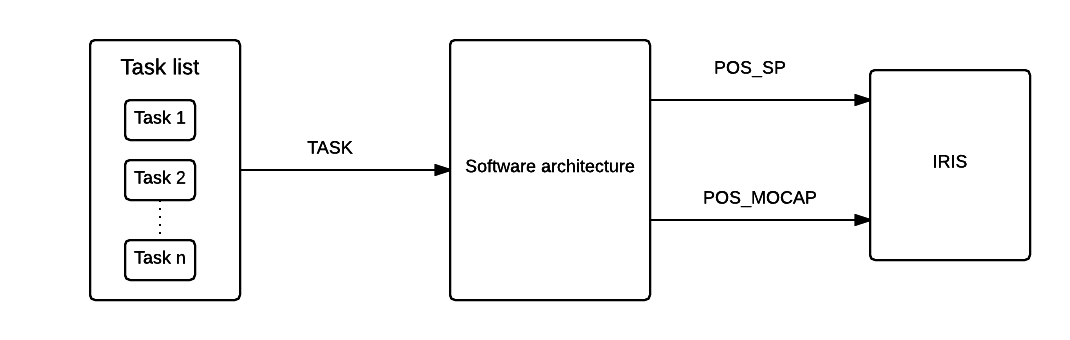
\includegraphics[width=0.8\textwidth]{first_arch.png}
 \caption[In-out relation]{Input / Output relation of the software architecture.}
 \label{figure:inout}
\end{figure}
The scheme explains the input output relation, where as input there is a C-struct describing the task and as output MavLink messages for mocap estimate and position set point. Nevertheless, the real structure is a bit different. I decided to put the task list inside the software architecture as a nested component. The main reason for that is simplicity, in the future one may encode the list in a text file as input of the software. See figure \ref{figure:inoutnest} for the actual implementation.

\begin{figure}[h]
\centering
 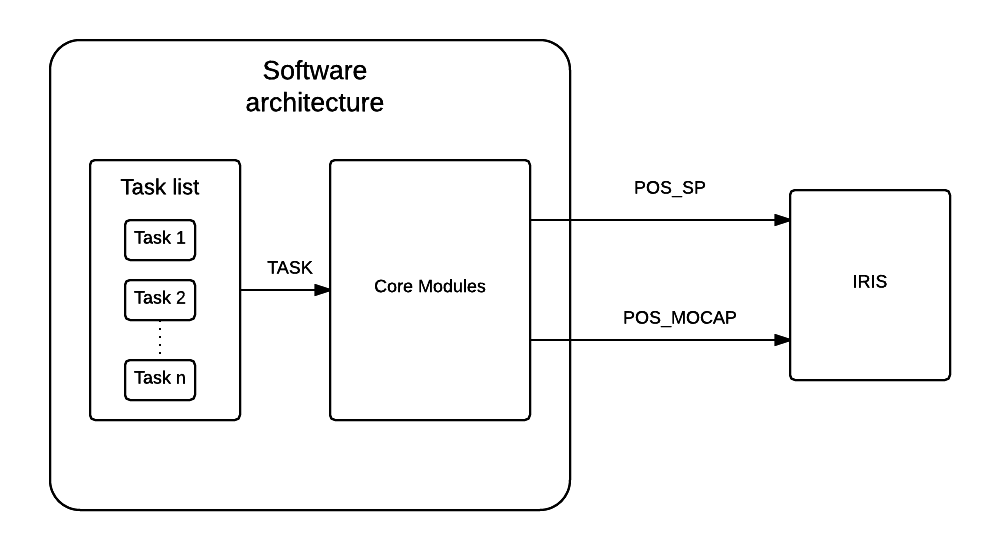
\includegraphics[width=0.8\textwidth]{nested_arch.png}
 \caption[In-out relation for the nested arch]{Input / Output relation of the software architecture with nested component.}
 \label{figure:inoutnest}
\end{figure}

\subsection{Behavioral architecture}
\label{sec:behav}
At this point, a way to model the problem is necessary. Let us start from the goal: there a list of tasks and the robot must executes them sequentially and autonomously. Thus, the concept of task arises. The task is defined as \textit{a definite piece of work assigned to the robot and performed by acting on the environment}. 

\paragraph{Defined tasks} Which kind of tasks may be performed by IRIS? The first step is to define the essential tasks of navigation which are:
\begin{itemize}
\item Take off - from the ground or an horizontal plane.
\item Land - land on actual position.
\item Move - go to a target point in 3-D space.
\item Rotate - Change yaw value to a desired one.
\item Follow trajectory - Perform a circle around an arbitrary center set in the parameters.
\end{itemize}
Moreover a fifth task is added but discussed in \ref{chap:seventh} which is land on a mobile platform. \newline \\
In order to make things more flexible, each task has a set of parameters used to influence the performance during the execution and to adapt to the environment. A detailed explanation is given in \ref{sec:auto}. Furthermore, it is evident that most of the tasks described involve in some way a location in space. Hence the task is modeled in a C-struct with two elements: position and action. In the software the task takes the name \textbf{node} which is often used in control stations and graph based applications.

Table \ref{tab:node} describes the node struct. The position \textit{p} is itself a struct with four elements (x,y,z,yaw) encoding the 4-D pose in space. The action \textit{a} is another stuct with a char value to identify the type of action and a parameter array which can be filled with values. The meaning of the parameter array changes depending on the action.
\begin{table}[h]
\centering
\begin{tabular}{llll}
\multicolumn{4}{c}{\textbf{Node} struct} \\
\hline
position \textit{p} &     &       &           \\
           & \textit{x}   & double & meters    \\
           & \textit{y}   & double & meters    \\
           & \textit{z}   & double & meters    \\
           & \textit{yaw} & double & radiants  \\ \hline
action \textit{a}   &     &       &           \\
           & \textit{id}  & char  &           \\
           & \textit{params}    &  double[4]     & \\
\end{tabular}
\label{tab:node}
\caption{Node struct descripton}
\end{table}
Those elements are necessary in order to choose which design pattern is suitable in this environment.
\newline \\
\noindent
Taking inspiration from biology and observing how simple animals interacts with the environment, robotic schemes and models may be derived. Biologist discovered that animals like frogs, pigeons insects and fishes exhibit different behaviors depending on the sensory inputs they receive from the environment. With this simple method they are able to survive, hunt and navigate. Two different examples explain the concept very well.

Frogs eyes are able to detect movement. In particular on layer detects small moving objects like flies and another layers detects big object, for example predators. The two layers work in parallel. When the first one is activated, meaning that there is food in the proximity, the frogs jumps towards the pray. On the other hand, when the second layer is triggered, the frogs run away from the object. 

The second example involves the navigation of pigeons. When it is sunny, the bird uses the sun to locate himself (behavior 1). When it is cloudy they use the magnetic field of the earth to detect the north (behavior 2). By disturbing the pigeon with artificial light, it get confused only in sunny days. Vice versa, if disturbed with a magnet, it get confused only in cloudy days. This simple experiment lead to an important result: the pigeon switch behavior depending on some triggering inputs just like the frog. More over only one behavior is active. 
\paragraph{Behavior definition} \textit{A behavior is a mapping of sensory inputs to a pattern of motor actions that are used to achieve a task.} \newline

\noindent
For the frog, the sensory inputs are be the position of the moving objects while for the pigeon they are the position of the sun and the value of the magnetic field. Moreover, a trigger is present. Those triggers are of different nature depending on the animal, they activate the behaviors or switch from one to the other. Figure \ref{figure:behavior} shows the basic model of the behavior. Inputs and output may be more than one while the activation trigger is always a single signal. 
\begin{figure}[h]
\centering
 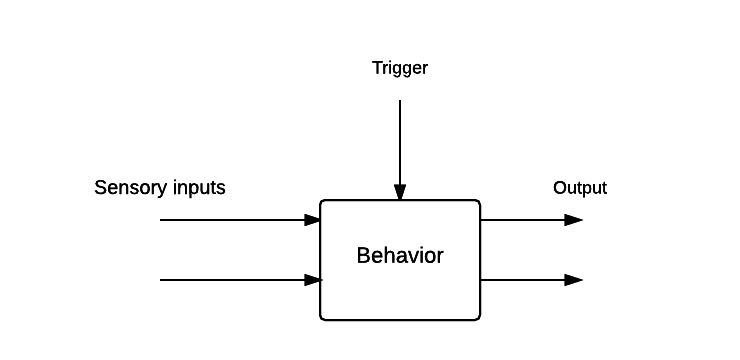
\includegraphics[width=0.8\textwidth]{behavior.png}
 \caption[Behavior definition]{Scheme of the behavior.}
 \label{figure:behavior}
\end{figure}
From an engineering point of view, imagine the behavior like a process, an algorithm, a thread or a module. Inputs and outputs may be variables, signals or parameters. The triggers are often booleans. The logic that manage the triggers is called \textbf{switching logic} and it is a key aspect in the architecture. The switching logic is usually a module that takes inputs from perception modules, and outputs the boolean values of each trigger. Figure \ref{figure:switch} describes a behavioral machine, n behaviors are connected to n trigger signals coming out from the switching module. The logic can be implemented in different ways. It could be a combinatorial circuit made by logical ports, some mathematical functions or a state machine but its output must be a set of n boolean values. 
\begin{figure}[h]
\centering
 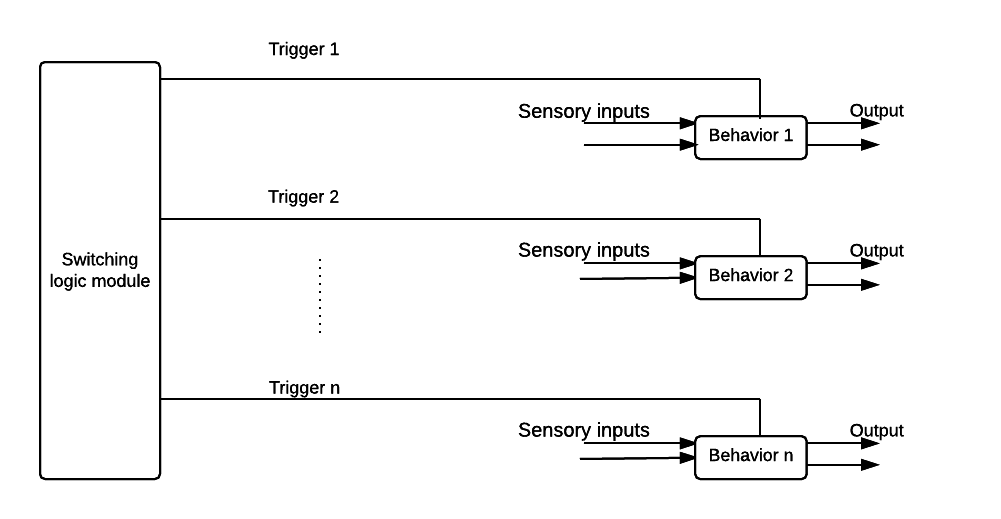
\includegraphics[width=0.8\textwidth]{switch.png}
 \caption[Switching logic]{Behavioral system with switching logic.}
 \label{figure:switch}
\end{figure}

\paragraph{Concurrent behaviors} One aspect I find very interesting is the concept of concurrent behaviors. Two or more behaviors are concurrent when they are active at the same time. This approach may solve elegantly different problems but we must pay some attention. Imagine the frog looking around. At some point an insect and a predator appear together in the field of view activating two behaviors. She is hungry, but more important, she does not want to be the meal of someone else. In this case behaviors can be prioritized (the most important is executed). A second way is to include this scene in the switching logic where behaviors inhibit others. Moving may inhibit landing for example. 

On the other hand let us picture the following situation: a mobile robot moving on the ground and going towards a target. The behavior \textit{move straight} is activated and the robot goes in the direction of the goal. At certain point the perception module senses an obstacle in front and activates the behavior \textit{avoid obstacle}. The two behaviors are concurrent since we assume that there is no inhibition in the switching logic. The first output is to spin the wheels with the same speed (move straight) but the second behavior commands the steering wheels to turn and avoid the collision. The to outputs add up and the result is the robot avoiding the obstacle. When the perception module does not sense anymore the obstruction, the second behavior is turned off and the robot continues moving towards the target. 

It seems pretty trivial but this approach has a lot of potential. It saves resources turning off and on different modules depending on the situation. Switching logic can be implemented on hardware thus optimizing the performances. Moreover the combinations of simple behaviors may solve complex tasks. 

For this case, in order to solve concurrency issues, I used a simple rule: \textbf{concurrent behaviors are possible only if they act on different dynamics}. For example, move and rotate can be activated together because one changes x, y and z while the other changes yaw set points. Follow trajectory and move cannot be concurrent because they act on the same dynamics. One may need to follow a trajectory, like a circle around a point of interest, and film with the camera the center thus keeping the nose always pointing to the target. This is solved combining \textit{follow trajectory} with \textit{rotate}. Although it is not implemented in this way, potentially the landing on a mobile platform task may be defined by two concurrent behaviors. The first is \textit{move} or track the platform, and the second is \textit{land}. The more behaviors are added, the more combinations are possible.

\paragraph{Implementing behaviors} The switching logic is implemented as a finite state machine which is presented in section \ref{sec:exec}. Behaviors are functions with the following inputs: the robot state (x,y,z,yaw), the actual position setpoint(x,y,z,yaw) and the node value. As output they give the new position setpoint which is updated. Figure \ref{figure:flow} shows the data flow for general set of behaviors, the switching logic is not shown for simplicity. 
\begin{figure}[h]
\centering
 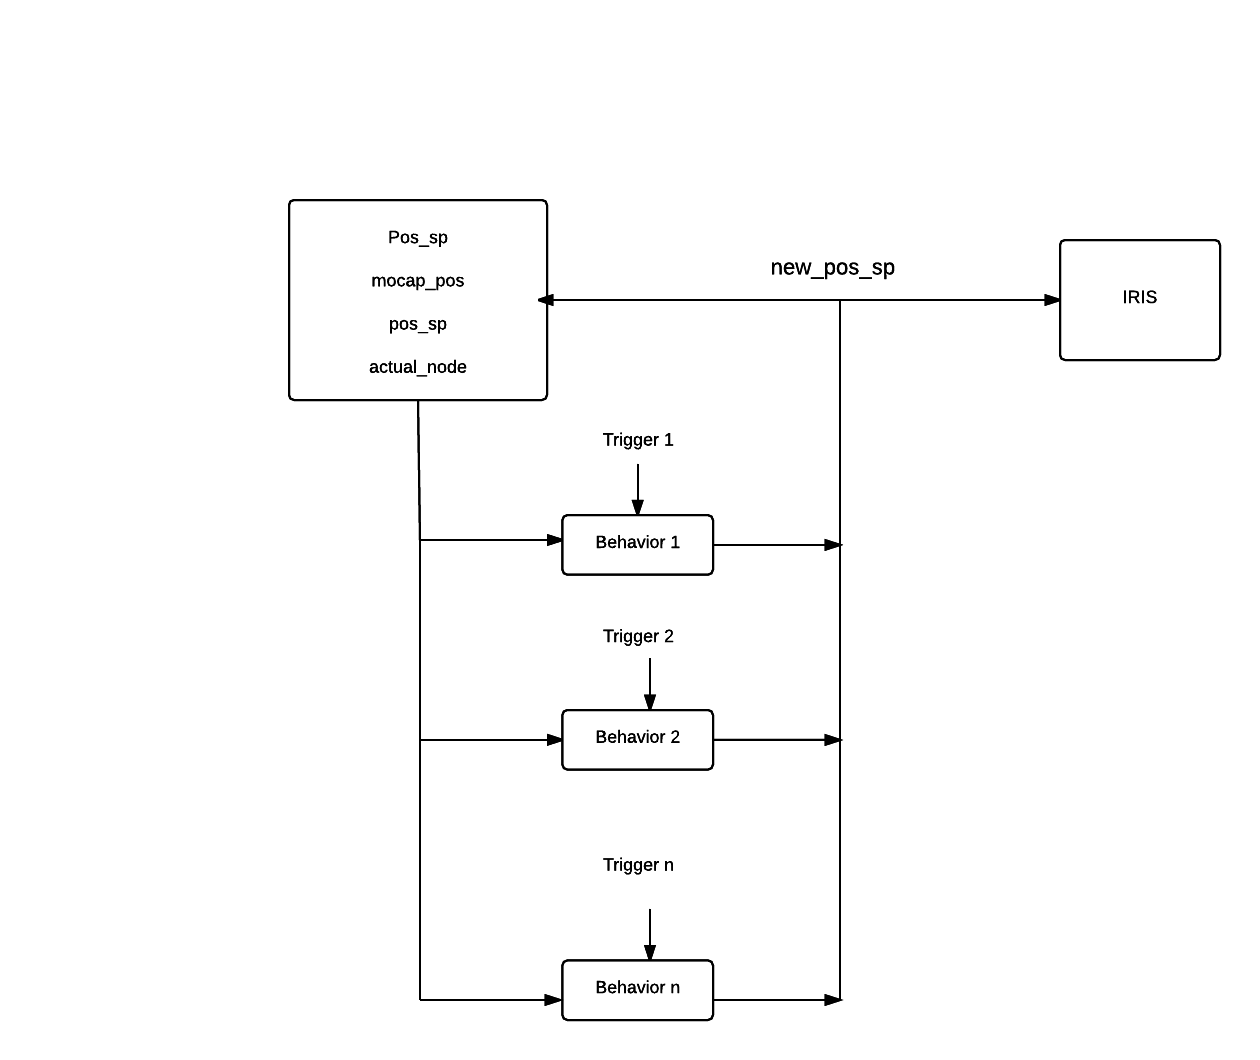
\includegraphics[width=\textwidth]{behav_flow.png}
 \caption[Behavior data flow]{Input/Output relations with particular adopted scheme. Switching logic is not depicted.}
 \label{figure:flow}
\end{figure}
Regarding implemented behaviors, the switching logic is almost a one to one map. Each presented task has its own behavior called with the same name. In this version of the software, the only concurrency appears in \textit{follow trajectory} task which performs a circle and keeps the nose always at the center. Depending on the actual task, the switching module activates different behaviors and the map is shown in table \ref{tab:map}.
\begin{table}[h]
\centering
\begin{tabular}{l|c}
Actual task               & Activated behaviors   \\ \hline
take off                  & take\_off             \\
land                      & land                  \\
move                      & move                  \\
follow trajectory         & follow\_traj ; rotate \\
rotate                    & rotate                \\
land on a mobile platform & plat\_land           
\end{tabular}
\caption{Switching logic mapping.}
\label{tab:map}
\end{table}

For prototyping and simplicity reasons, the mobile landing has its own behavior but two concurrent behaviors can be assigned to it, namely \textit{move} and \textit{land}. Moreover, many improvements can be done. For example one can decide to activate or not the \textit{rotate} behavior in the follow trajectory task by passing a value in the params array. This architecture can be largely expanded from its actual state by adding behaviors, concurrencies and tasks.



\section{Software description}
\label{sec:sofdescrip}
At this stage, the actual implementation of the concepts explained previously can be described. The structure of the application is a multi-threaded scheme. A thread of execution is a sequence of programmed instructions that can be managed independently by a scheduler. Different threads implement different modules or processes running simultaneously and independently. Within the Qt environment, multi-threading is easily implemented through the QThread class. By inheriting its properties we can redefine its \textit{run()} method and design the wanted algorithm. The advantages of having a multi-threaded architecture are several. Threads can be started and stopped as many times we need. Moreover, if a thread fails or get stuck, the others continue running since they are all independent. This is a key aspect in consideration of the fact that there are essential modules which cannot be blocked by other threads. 

This scheme presents also a main drawback. When two or more threads are running in parallel, they may need to access to the same variable. As result they could interfere with each other, thus synchronization is essential and some precaution is a must. 

To summarize, we can write threads by inheriting properties by the QThread class and overloading its \textit{run()} function with our custom code. By calling the start method, the thread is started and \textit{run()} is executed, usually an infinite loop is implemented with a custom rate. Each loop runs in parallel, hence if one gets stuck the others continue spinning. 

Another powerful tool is the connect method. This method is member of each class in Qt since they are derived from the same one. Every class has signals and slots. Slots are just methods while signals are booleans. With connect, we can relate the signal of one class with the slot of another class. Meaning that, if the signal of the first class at certain point goes up then the slot of the second class is executed. It can be done within threads so callbacks can be partially simulated. 
With this first overview, the reader should have a rough idea on the working principle of the system. Infinite loops are running simultaneously and independently and each one represent a module. The following custom module are implemented, they represent the main ingredients and the core of the application: \begin{itemize}
\item NatNet Reciever
\item Position Dispacher 
\item Manual Control
\item Automatic Control 
\item Executioner
\item Commander
\end{itemize}
The \textit{NatNet Reciever} and \textit{Position Dispatcher} are also called service module. The Reciever task is to read the value of the mocap estimate and save it on a global variable. The Dispatcher takes the estimate and the position set point, packs them in MavLink messages and send them trough a socket interface via usb to the radio module. 

\textit{Manual Control} module incorporates an user interface through which the user can change manually position set point during flight. It runs on the same thread of the service modules, namely the main thread which is created at the starting of the entire application. 

\textit{Automatic Control} stores the algorithms for every behavior and execute them depending on the switching logic. It is the central member of the application.

\textit{Executioner} module implements the switching logic as a finite state machine.

\textit{Commander} is the lower level module. It is the only one which has the permission to update the position set point value.

\paragraph{Communication} Communication between modules is done with a simple method. Every common data is stored as a global variable. Producers update the variable while consumers read it from the global space. This approach is not optimal but very simple to implement. With the use of the QMutex class we are able to lock and unlock variables in the read/write operations.

\paragraph{Note: } service modules were previously implemented by Tommaso Falchi Delitalia, in his PhD work, and slightly modified by me in order to adapt them with the rest of the application.

\subsection{General scheme}

More technical details can now be presented. As already mentioned, the design started with service modules implemented. In that implementation the communication management with global variables was used and I continued on that direction. 

\paragraph{Implementation} The actual implementation is explained in this section. First of all, let us introduce the class MavState. This class is used to store mocap values and position set points. The elements of the class are 3 coordinates of the position in space, 4 values for the quaternion orientation and one value for the yaw in radians. The class with members and methods is shown in table \ref{tab:mavstate}.
\begin{table}[h]
\centering
\begin{tabular}{llll}
members &                        &                                                      &            \\
        & x , y , z              & position in 3D space                                                                                        & meters     \\
        & yaw                    & value for the yaw                                                                                           & radians    \\
        & qw , qx ,qy qz         & values for the orientation                                                                                  & quaternion \\ \hline
methods &  & &  \\
& setPosition(x,y,z)     & set values for the position                                                                                 &            \\
        & setOrientation()       & \begin{tabular}[c]{@{}l@{}}set values for orientation passed like \\ quaternions or RPY angles\end{tabular} &            \\
        & getPosition(x , y , z) & get value of position                                                                                       &            \\
        & getOrientation()& get value of quaternion or RPY angles                                                                                                             &           
\end{tabular}
\caption{MavState Class}
\label{tab:mavstate}
\end{table}

\begin{figure}[h]
\centering
 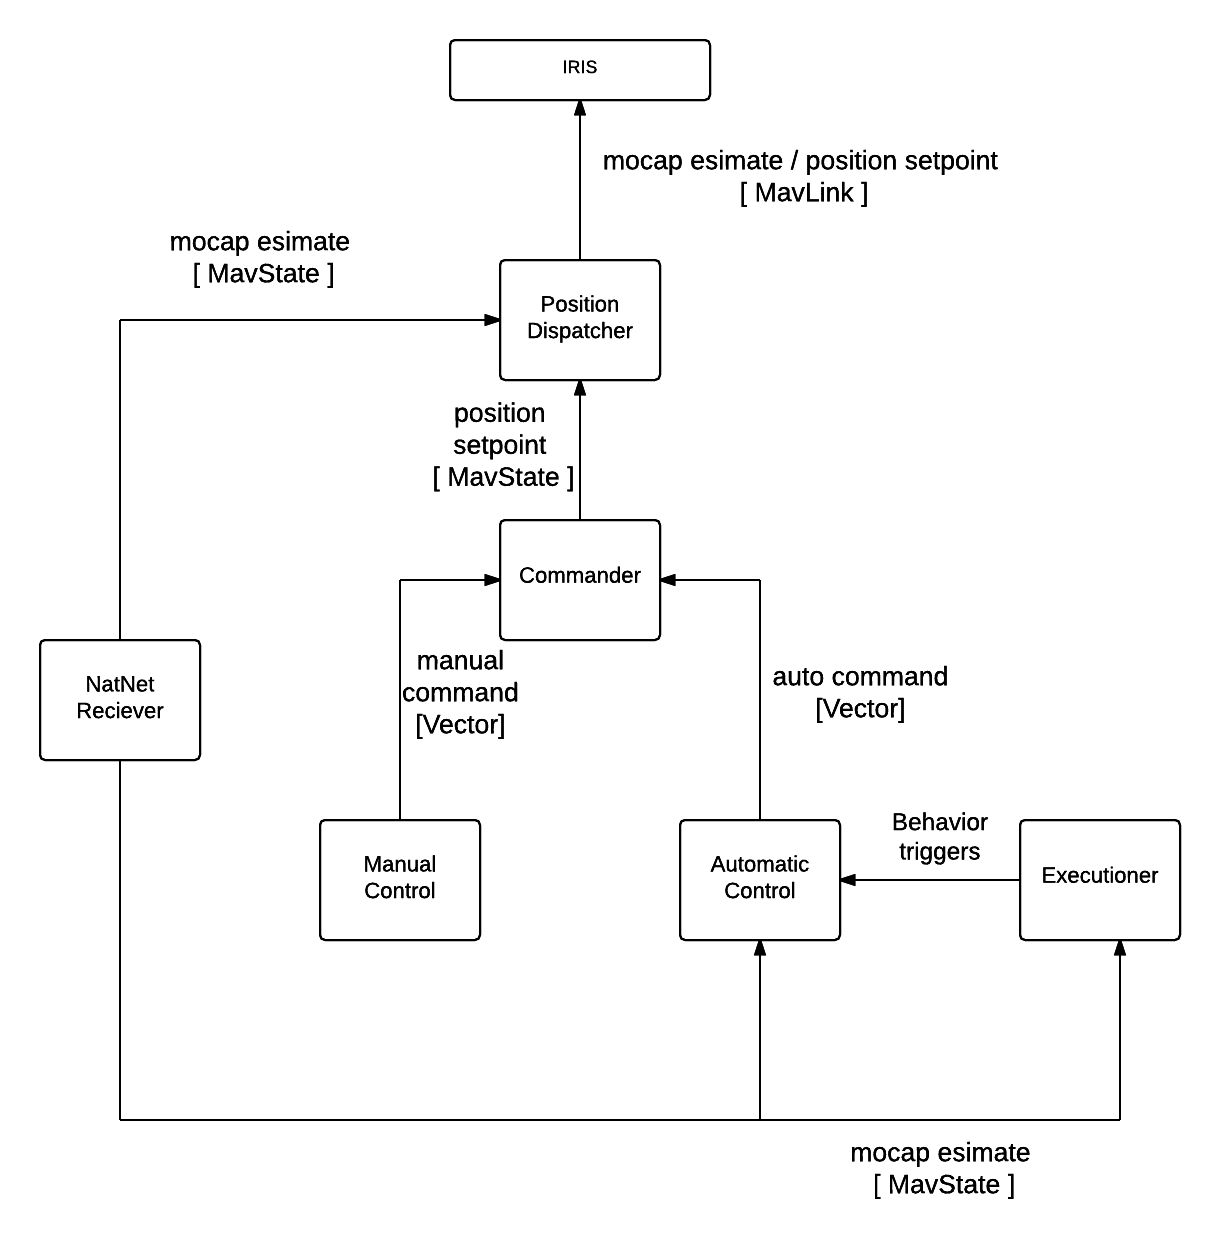
\includegraphics[width=0.9\textwidth]{arch_scheme.png}
 \caption[Achtitecture scheme]{Implementation of the system.}
 \label{figure:archscheme}
\end{figure}
The full scheme is represented in figure \ref{figure:archscheme}. We must give some consideration on the implementation of system. The mocap estimate is saved in a MavState global variable, potentially every module may access it. The used entries are position (x , y , z) and yaw (retrieved from quaternion).

The automatic Control implements the behavioral part and calculates a new position set point (position and yaw). The new setpoint is pushed in a vector called auto command. In the same way, Manual control pushes the new set point in the manual command vector. The Commander module checks both vector and evaluate which command is good to be sent. This rule is used: \textbf{if the two vectors are non empty, then the command sent will be the one in the manual vector}. It basically prioritize the manual command over the automatic ones and update the position set point in the global space. The executioner implements the switching logic; according to the actual state of the robot and the actual action to be performed it decides whether stay in the same node or switch to the next one. It then updates the values of every triggering signal which are saved in the global space.

For sake of clarity, in figure \ref{figure:archscheme} messages are represented by arrows. The connections are only logical because potentially every module can access those signals since they are stored in global space. In addition, the node list defined by the user and the id of the actual node which is executing are stored globally.

\subsection{Service modules}

Those modules run on the main thread and they use the signal/slot feature embedded in Qt. 

\subsubsection*{NatNet Reciever}

Using the proprietary SDK from NaturalPoint, this module parses the position of the center of mass and the orientation of every rigid body tracked by motive. In the actual state of implementation, only two bodies are saved. The value is saved in MAvState classes contained in the  namespace \textit{g} with the following convention: \begin{itemize}
\item Rigid body number 1 is saved in g::state 
\item Rigid body number 2 is saved in g::platform
\end{itemize}
The order is very important, the robot must be labeled as one and the mobile platform as two. This is easy to check with motive. Every time g::state is saved, the signal dataUpdate is emitted.
\subsubsection*{Position Dispatcher}

The signal dataUpdate is connected to the slot sendPosition() of the Position Dispatcher. As consequence, every time the robot state is updated, sendPosition() is executed. This function takes the state and the postition setpoint (saved by the commander in g::setPoint variable) and fills two mavlink packages. The state MavLink package is predefined for Optitrack, while for the set point I used the Vicon dedicated package. The same message cannot be used since PX4 creates a uOrb topic for each mavLink type received, thus they would be written on the same topic. 

When the messages are ready, trough a socket interface, they are sent to the radio module. The radio has a dispatch interval of 100 ms, meaning that after sending data, we must wait 100 ms. If messages arrive in this interval they are ignored. 

\subsection{Manual Control}

\begin{figure}[h]
\centering
 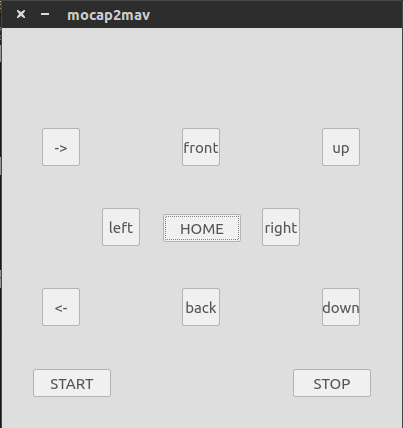
\includegraphics[width=0.4\textwidth]{mangui.png}
 \caption{Manual user interface.}
 \label{figure:mangui}
\end{figure}

Manual Control is started at the beginning in the main thread. It features a simple user interface shown in figure \ref{figure:mangui} which translates the position set point on three axis and rotates th yaw. The home button issues a setpoint in the center of the room. The starting setpoint is $[0,0,-1]$ for position and $\pi$ for the yaw. Thus, \textbf{the robot must be placed on that location} on the horizontal plane and yaw if one wants to fly it by manual control. If not placed correctly, the take off could be dangerous. The start and stop button run an auxiliary thread which I used for prototyping and testing. 

Each time the user click on a translational button, the set point is moved by $0.1$ meters on that direction in earth frame. The yaw is changed by steps of $\pi/18$ radians.


\subsection{Automatic Control}
\label{sec:auto}
This module is the core of the application. It implements the behavioral pattern explained in section \ref{sec:behav}. It is defined with the class \textit{Automatic} and it has one member: \textit{AutoThread}. This thread implements a \textit{run()} function which is started by clicking on the button AUTO. The loop runs at 10 Hz. When the thread starts the system is in automatic mode, thus it executes the nodes present in the list (stored globally) in succession. Every behavior is implemented as a function and the structure of the loop is:
\begin{algorithm}
\begin{algorithmic} [1]
\WHILE{true}
\STATE{$comm = g::setPoint$ } \COMMENT{save previous set point}
\IF{take\_off\_sig}			  
\STATE{$take\_off();$}
\ENDIF
\IF{move\_sig}			  
\STATE{$move();$}    
\ENDIF
\IF{land\_sig}			  
\STATE{$land();$}
\ENDIF
\IF{rotate\_sig}		  
\STATE{$rotate();$}
\ENDIF
\IF{follow\_traj\_sig}			  
\STATE{$rotate();$}
\STATE{$follow\_traj()$}
\ENDIF
\IF{land\_plat\_sig}			  
\STATE{$land\_plat();$}
\ENDIF
\STATE $autoCommand.pushback(comm)$ \COMMENT{fill the command vector}
\STATE publish()
\ENDWHILE
\end{algorithmic}
\label{alg:autothread}
\caption{Brief overview of the automatic thread.}
\end{algorithm}
The structure is simple, while spinning, we read each value of <\textit{task>\_sig} coming from the switching logic and activate different portion of code. In particular, we run specific functions depending on the behavior. Those function modify the $comm$ variable which is then published in the command vector. The signal publish() at line 23 is connected with the commander slot which is asked to check to check the command vectors. 

At this point we can explore deeply how behaviors are implemented.

\paragraph{Take off} Taking off is pretty simple. When the behavior is activated for the first iteration, it saves the actual horizontal position and yaw. Then a set point is issued on the vertical of the starting position at a fixed altitude with the initial yaw. 

\paragraph{Move} 

\begin{figure}[h]
\centering
 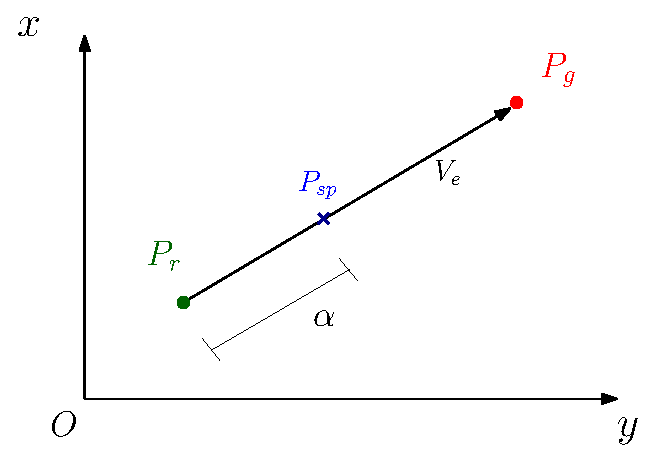
\includegraphics[width=0.4\textwidth]{move1.eps}\hspace{0.1\textwidth}
 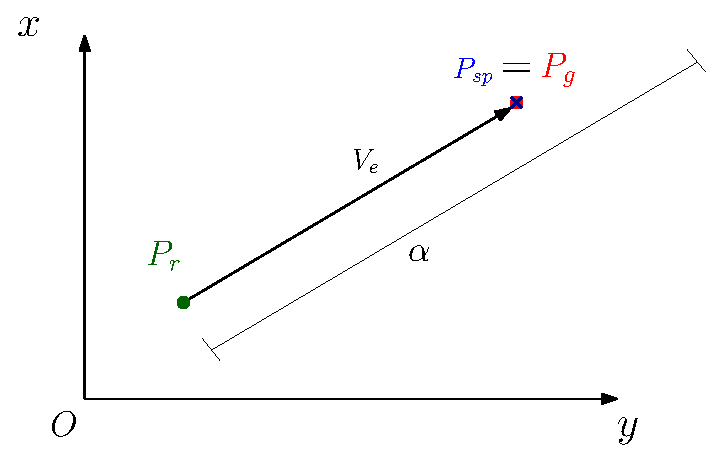
\includegraphics[width=0.4\textwidth]{move2.eps}\\[1em]
 \caption[Move function.]{Move function. On the left the limited position set point in blue, on the right the case with no scaling.}
  \label{figure:move}
\end{figure}

The move action is a bit more complex. At each loop spin the 3D position error is calculated, namely the difference between the goal and the actual position.  This difference results in a vector $\boldsymbol{V_e} = \boldsymbol{P_g} - \boldsymbol{P_r}$ originating on the robot position $\boldsymbol{P_r}$ and going towards the goal $P_g$. Let us define a positive constant $\alpha$ and let $\boldsymbol{u_e} = 	\frac{\boldsymbol{V_e}}{\lVert\boldsymbol{V_e}\rVert}$. Then the following method is used to calculate the position set point $P_{sp}$ to be sent to the commander: 
\begin{equation}
\boldsymbol{P_{sp}} = 
\begin{cases}
    \boldsymbol{P_g}, & \text{if } \lVert\boldsymbol{V_e} \rVert \leq \alpha \\
    \boldsymbol{P_r} + \alpha \boldsymbol{u_e},&    \text{if } \lVert\boldsymbol{V_e}\rVert > \alpha
\end{cases}
\label{eq:move}
\end{equation}
The principle of this function is depicted in figure . The reason why we limit the position set point is because of the effect of the proportional term in the position controller. Issuing a far set point, the error is high and the desired velocity becomes big. Hence, in order to avoid this kind of effect, which results in bad flight dynamics, we limit the distance of the issued position set point from the robot by a distance $\alpha$.

\paragraph{Land} Landing maneuver consists in slowly increasing the z (the z axis is upside down, increasing z the height decreases) while maintaining the horizontal coordinates of the last position set point(where the robot is). Thus, only z coordinate of g::setPoint is changed. The trick used simulates  kind of velocity control. The z coordinate of the set point is calculated depending on the horizontal error between the robot and the vertical of the target landing point and it is given at a fixed vertical distance with the robot. That means that when the robot descend, the set point maintain a fixed distance with robot position. This results in a fixed vertical error an a constant vertical velocity. Let $h_e$ being the horizontal error of the robot from the landing vertical and $P_r(3)$ the z coordinate of the robot, then the following empirical value are found to be good:
\begin{equation}
z_{sp} = 
\begin{cases}
    P_r(3) + 0.3 , & \text{if } 0.5 <  h_e\ \leq 0.8 \\
    P_r(3) + 0.5  , & \text{if }  h_e\ \leq 0.5
\end{cases}
\label{eq:land}
\end{equation}
When the height of the robot is sufficiently small, the rotor are set to idle by issuing a set point under the ground and the robots land. Note that the vertical set point sums up with the robot position because z axis is pointing towards earth. Moreover, horizontal set points are slightly compensated in order to increase precision. Let $\boldsymbol{P_t} = [x ,y]^T$ the landing target on the horizontal plane and $\boldsymbol{P_{sp}} = [x_{sp} ,y_{sp}]^T$ the actual set point command, then the compensation is the following:

\begin{equation}
\boldsymbol{P_{sp}} = \boldsymbol{P_t} + K_p\boldsymbol{e_p}
\end{equation}
Where $K_p$ is the correction gain and $\boldsymbol{e_p} = \boldsymbol{P_t} - \boldsymbol{P_r}$ with $\boldsymbol{P_r}$ the robot horizontal position. In this way we increase the landing precision emulating an increase on position gains.

\paragraph{Rotate} Rotate action is done by sending yaw set points in radians. Let us define two functions: \textit{increase\_yaw()} and \textit{decrease\_yaw()}. The actual implementation is not discussed but a brief presentation is given. The first function issue a yaw set point which is equal to the actual yaw plus a delta (rotate a bit clockwise), on the other hand \textit{decrease\_yaw()} rotate a bit counterclockwise. With those two elementary methods we can design an algorithm which, given a generic yaw set point in radians, rotates the robot in the direction which spans the smallest angle to the target. 

Firs of all, we must recall few concepts. In section \ref{sec:trasfmatrix} the yaw angle is defined as $-\pi < \psi < \pi$. Imagine a top view of the earth frame with x axis vertical and going upwards and y axis horizontal pointing to the right. The yaw is the angle is positive on the right half of the plane and negative on the left half. This property works also in body frame meaning that: each direction on the right side of the robot has a positive yaw and each direction on the left side of the robot has a negative yaw (in body frame, be careful). Positive yaw in robot frame means a clockwise rotation while negative yaw means a counterclockwise rotation (we have functions for that). 

That said, the idea is simple. First we express the desired direction (yaw set point) in robot frame and then we check whether it lies on the right or left side by looking at the yaw sign. For expressing these procedure in equations let $R_z(\psi)$ be the rotation matrix on z by an angle $\psi$ and $\boldsymbol{V_{sp}^E} = [\cos(\psi_{sp}),\sin(\psi_{sp}),0]^T$ a unit vector encoding the desired direction in earth frame calculated from the yaw set point $\psi_ {sp}$, then the desired direction in body frame is:
\begin{equation}
\boldsymbol{V_{sp}^B} = R_z(\psi) ^T \boldsymbol{V_{sp}^E}
\end{equation}
where $\psi$ is the actual yaw of the robot. Next step is to extract the yaw of the vector $\boldsymbol{V_{sp}^B}$ which is expressed in body frame by the following expression:
\begin{equation}
\psi_{sp} ^ B = atan2(V_{sp}^B[1],V_{sp}^B[0])
\end{equation}
if $\psi_{sp} ^ B > 0$ it means that the shortest path to point at the desired yaw is to rotate clockwise, otherwise the rotation is counterclockwise. Figure \ref{figure:rotate} shows the quantities involved in the procedure. In the case of the figure we have a negative desired yaw in earth frame but positive in body frame. That means that the shortest path is clockwise and it is easily verifiable just looking at the image.

\begin{figure}[h]
\centering
 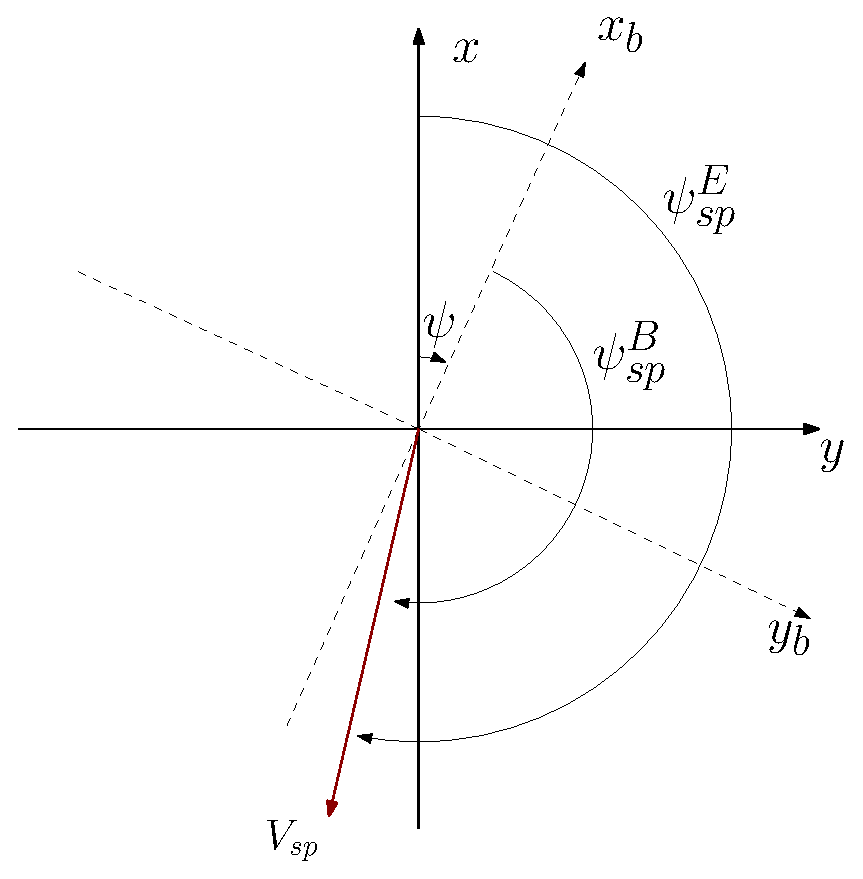
\includegraphics[width=0.8\textwidth]{rotate.eps}
 \caption{Involved frames in rotation task.}
  \label{figure:rotate}
\end{figure}
Moreover, the yaw set point can be provided in radians or  as a directional vector.


\subsection {Executioner}
\label{sec:exec}
The last component is the Executioner. This module implements the switching logic and it contains the definition of each nodes. It is defined by a class with one member: ExecThread. This thread is started together with the automatic thread and it runs a loop until all the tasks are performed. The position of the actual node is stored in an integer variable $i$ in the global space. At the beginning $i = 0$, the executioner increases this variable every time an action is completed. The automatic thread reads $i$ and looks in the list what is the actual node, from which it reads the value of position and parameters. Those value correspond to the sensory inputs of the activated behavior.

\begin{figure}[h]
\centering
 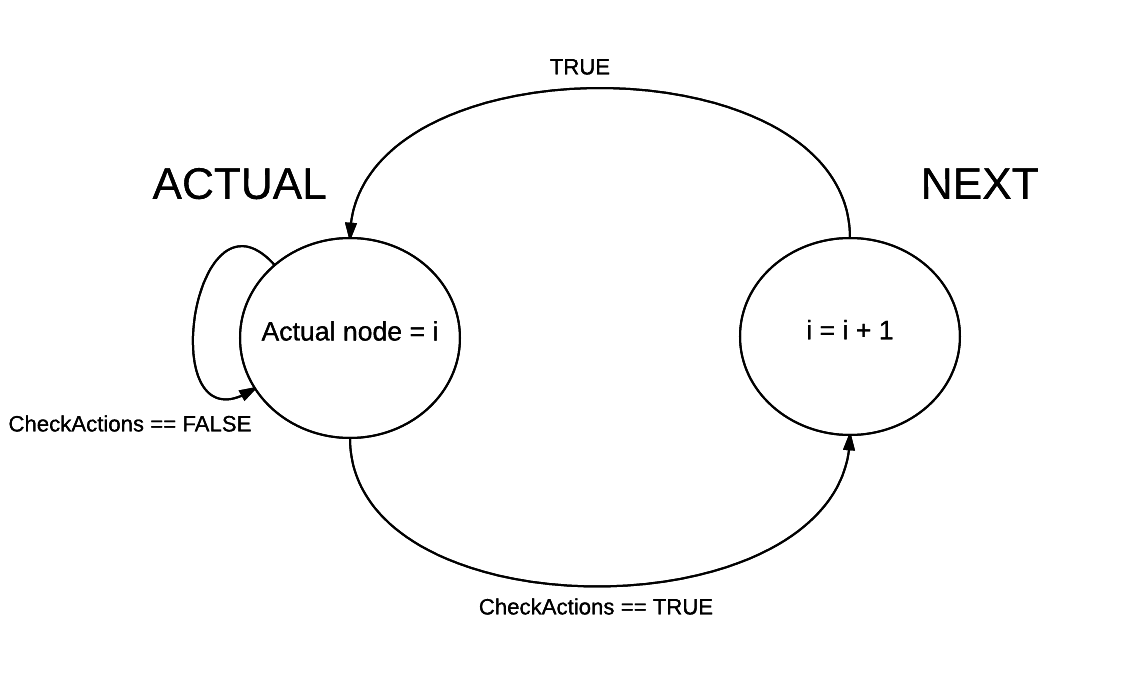
\includegraphics[width=0.8\textwidth]{executioner.png}
 \caption[Executioner sate machine.]{State machine diagram of the executioner module.}
  \label{figure:exec}
\end{figure}
 
This process can be explained clearly using a state machine diagram. The machine has two states, one is called \textit{ACTUAL} in which the output is the actual value $i$ and the other is \textit{NEXT} in which $i$ is increased by 1, meaning that we can pass to next node. The initial state is \textit{ACTUAL}; until the function checkActions() returns false, the state remains the same. When checkActions() returns true the state changes to \textit{NEXT}, \textit{i} is increased and then it switches back to \textit{ACTUAL}. Those operations are done at 10 Hz. The function \textit{checkActions()} reads the actual state of the system and, depending on the actual action, checks a number of stopping conditions (i.e. when te robot is near the target point, move task finishes. When the vertical velocity is zero and the robot is close to the ground, land task is performed.) returning ture if they are satisfied, false otherwise. 

The state machine relies on boolean signals to communicate with other modules. Those signals are organized in global namespaces, one for each action. For example, the namespace \textit{executioner::move} has two important boolean members: one is \textit{move\_sig} and the other is\textit{ move\_done}. The first one correspond to the behavior trigger (see algorithm \ref{alg:autothread}), this signal is set to true when the index $i$ points to a node in which the move action is encoded, to false otherwise. Figure \ref{figure:exec} explains those concepts. 

Informations on actions are given in table \ref{tab:actions}.

\begin{table}[h]
\centering
\begin{tabular}{l|cl}
Action            & id (char) & parameters (double{[}4{]})                                                                              \\ \hline
take off          & 't'       & params{[}0{]} = final height                                                                            \\ \hline
move              & 'm'       & \begin{tabular}[c]{@{}l@{}}params{[}0{]} = alpha\\ params{[}1{]} = hovering time on target\end{tabular} \\ \hline
rotate            & 'r'       & params{[}0{]} = angle valid                                                                             \\ \hline
land              & 'l'       & \begin{tabular}[c]{@{}l@{}}params{[}0{]} = touchdown speed\\ params{[}1{]} = ground height\end{tabular} \\ \hline
follow trajectory & 'c'       &                                                                                                        
\end{tabular}
\caption{Actions coding and parameters}
\label{tab:actions}
\end{table}


\section{Experiments and results}

The first experimental stage was to test each behavior singularly, after some more complex node lists were tested successfully. 

The performances of the task rotate and take off are already presented in section \ref{sec:conresults}. Figure \ref{figure:zconv} shows the take off maneuver; as already pointed out, the response is very slow at the first takeoff of the flight since the saturation of the integral on z axis, which compensates for gravity, is pretty slow. Figure \ref{figure:yawconv} show the rotation maneuver in which a constant yaw rate is implicitly set being the yaw set point a line over time. The convergence is very good. 

The move behavior is also partially tested and analyzed in section \ref{sec:conresults}. Figure \ref{figure:xconv} and \ref{figure:xconv} shows the move maneuver with no scaling factor $\alpha$ but what happens if we introduce it? The expectation is to see the set point with the shape of a ramp depending on the scaling factor value. Four move nodes were placed in the node list (beside take off and land), each node is the vertex of a square centered in (0,0) with the edge 1.6 meters long. Image \ref{figure:xalpha1} shows the move function with the scaling term $\alpha = 1$ while figure \ref{figure:xalpha06} represent the same experiment with $\alpha = 0.6$. 
\begin{figure}[h]
\centering
 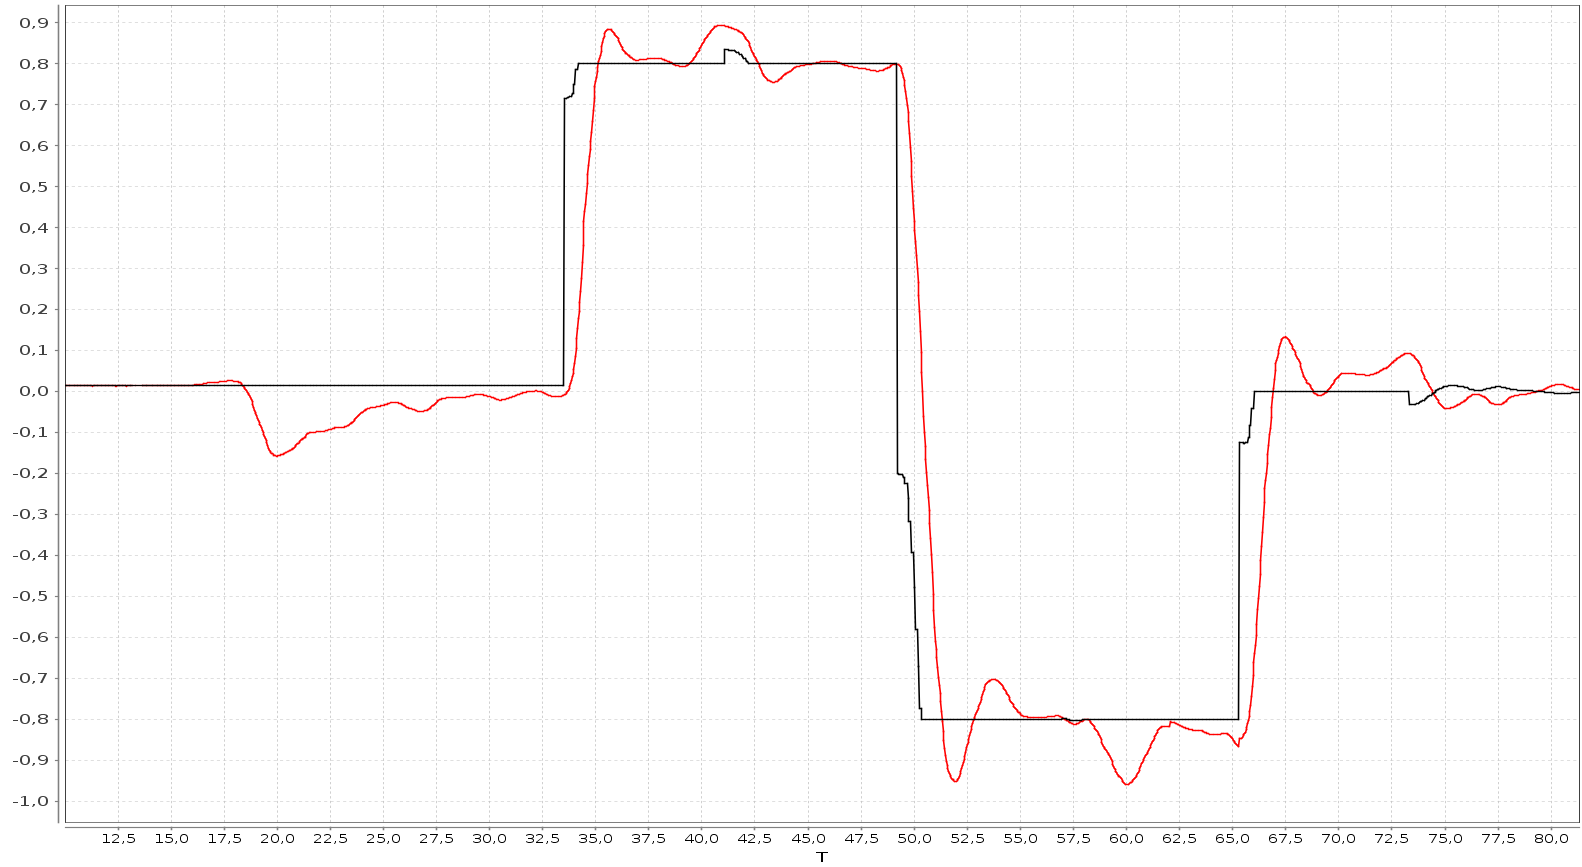
\includegraphics[width=0.8\textwidth]{xalpha1.png}
 \caption{Move with alpha 1}
 \label{figure:xalpha1}
\end{figure}

\begin{figure}[h]
\centering
 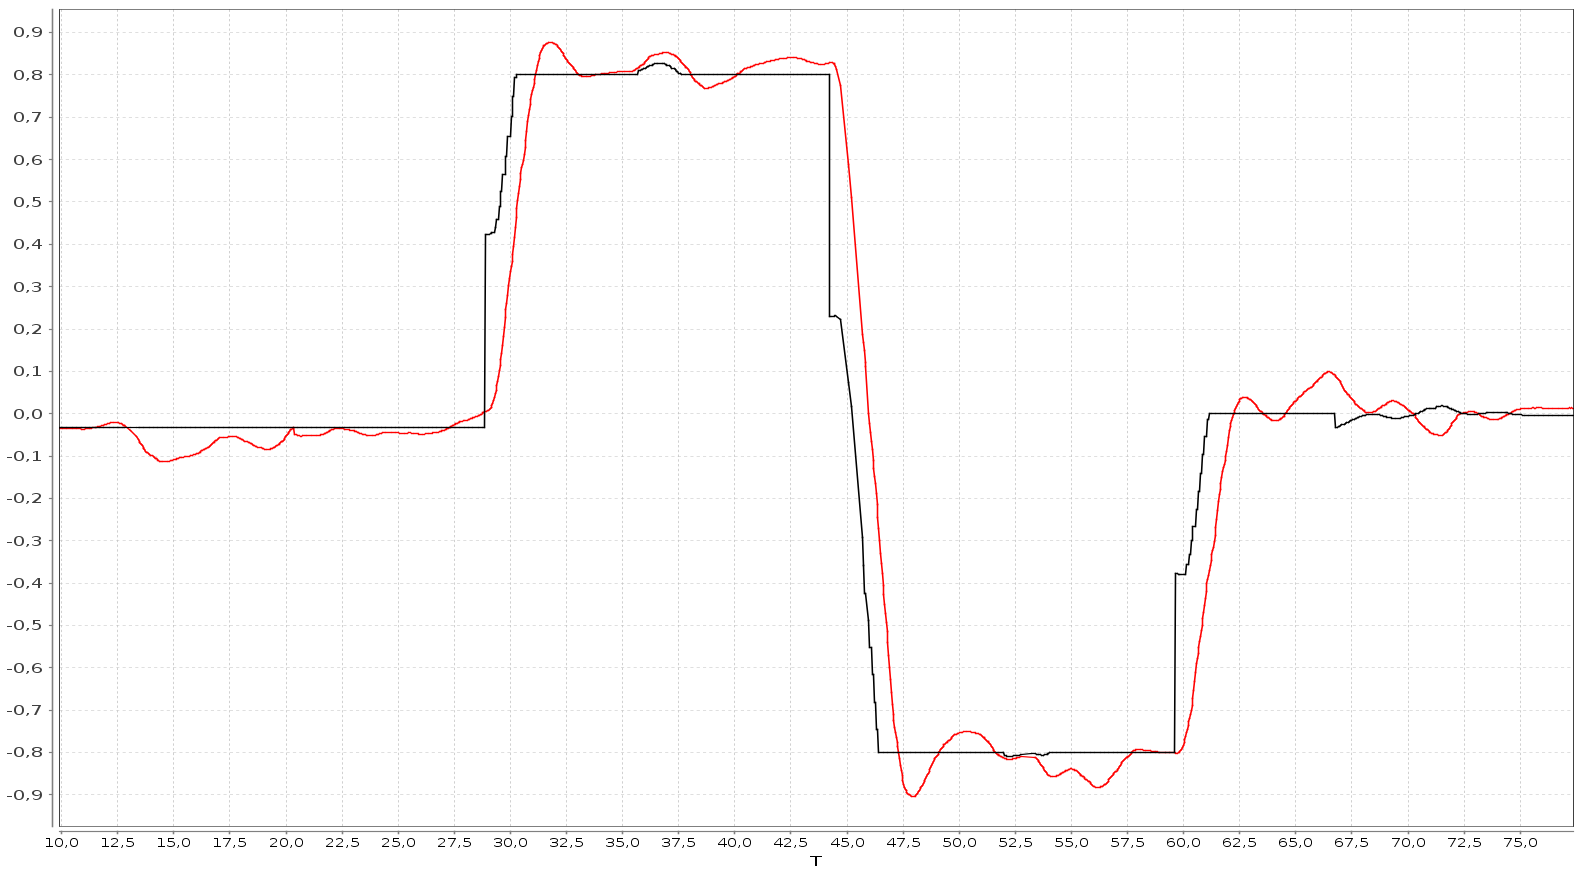
\includegraphics[width=0.8\textwidth]{xalpha06.png}
 \caption{Move with alpha 0.6}
 \label{figure:xalpha06}
\end{figure}
We can easily see the difference between the two experiments. The gap between the position and the set point is bigger with higher scaling factor but the maneuver is faster with more oscillations. The small oscillations of the  set points are due to the fact that the error takes into account the robot position, which oscillates by definition inducing this phenomenon. From second 65 the landing procedure begins, the oscillations of the set point the set point compensation for more accuracy explained in the landing section. Figure \ref{figure:takeland} show the altitude profile, from take off to landing, during previous experiments. 

\begin{figure}[h]
\centering
 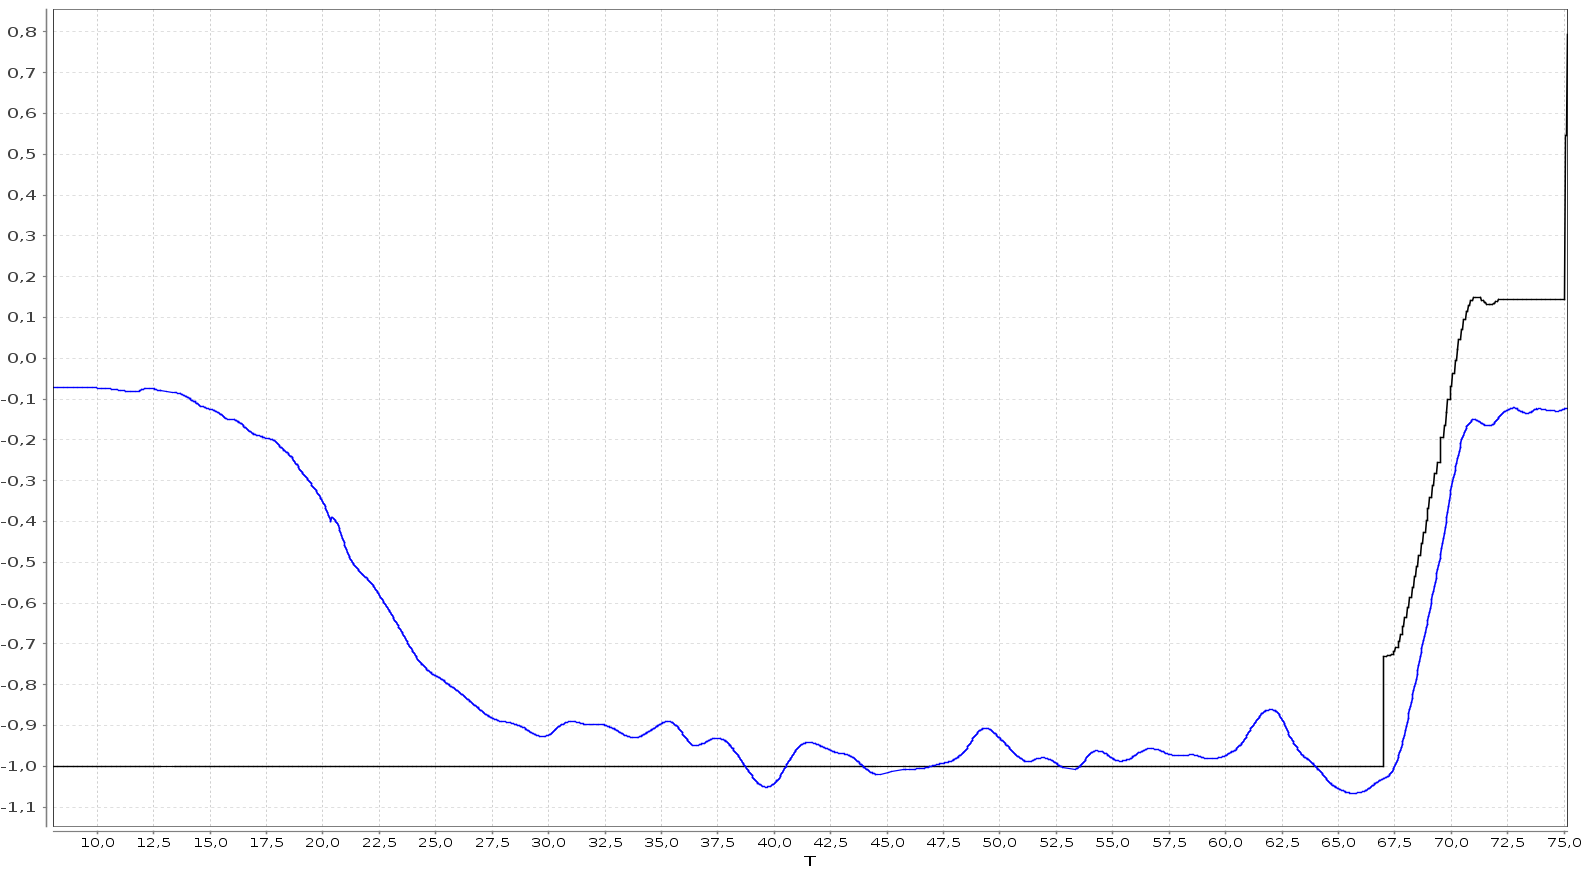
\includegraphics[width=0.8\textwidth]{takeland.png}
 \caption{Height profile}
 \label{figure:takeland}
\end{figure}

This experiment validates two aspects. The move function works as expected but, more important, the procedure is done autonomously validating the whole architecture at least for simple node lists. 

% % pure y e z?

Next experiment evaluates the landing precision. We let the robot take of, reach a point and land. This for forty times in different directions. After each land the horizontal error was measured and the results are reported in figure \ref{figure:takeland}. The mean error is about $-0.005$ on x and $-0.01$ on y for both axis, more than acceptable for landing precisely on different platforms.


% % METTI GRAFICO MATLAB

The third experiment is qualitative. We let the robot take off, land on a table, take off again and land on another platform with different height. This procedure is done just by filling the node list and set nodes parameters properly. Platform height were measured with the mocap. The result video can be viewed here \url{https://www.dropbox.com/s/vsub85qwvnx45um/multiland.MP4?dl=0 }. 

The last experiment consists in a more complex lists which incorporate every designed behavior. The output of the program is shown in figure \ref{figure:snip} where we can see every successfully node executed. The full video can be viewed here \url{https://www.dropbox.com/s/41kpdlm5svm9iir/circle_final.MP4?dl=0}. 

\begin{figure}[h]
\centering
 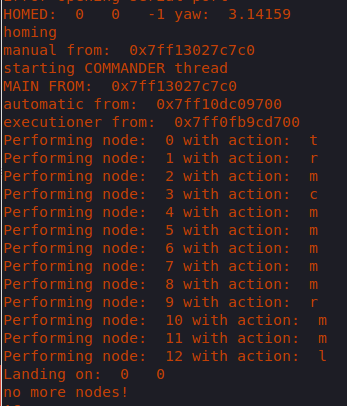
\includegraphics[width=0.5\textwidth]{snippet.png}
 \caption{Output for the last experiment}
 \label{figure:snip}
\end{figure}













